\documentclass[a4paper,12pt]{article}

\usepackage[english]{babel}
\usepackage{graphicx}
\graphicspath{{figures/}}

\setlength{\textheight}{243 mm}
\setlength{\textwidth}{16.3 cm}
\setlength{\oddsidemargin}{-0.5 cm}
\setlength{\topmargin}{-1.0 cm}
\setlength{\evensidemargin}{-0.5 cm}

\begin{document}

\begin{center}
  {\Large\bf Investigation of charge exchange reaction in deuteron-proton
    interaction at the Nuclotron.} \\

  {\large\bf  (STRELA collaboration.)}
\end{center}
{\large\bf
  V.A.Arefiev$^{1}$, I.Atanasov$^{2}$, S.N.Bazylev$^{1}$, G.N.Berezin$^{1}$,\\
  Yu.T.Borzunov$^{1}$, Yu.P. Bushuev$^{1}$, V.V. Glagolev$^{1}$,
  L.B.Golovanov$^{1}$, D.A. Kirillov$^{1}$,
  P.P.Korovin$^{1}$,  V.L.Lyuboshitz$^{1}$,  P.K.Maniakov$^{1}$,\\
  G. Martinsk\'{a}$^{3}$,
  E.A.Matyushevsky$^{1}$, N.S.Moroz$^{1}$, J. Mu\v sinsk\'y$^{3}$,
  B. Pastir\v c\'ak$^{4}$,
  N.M. Piskunov$^{1}$, A.A.Povtorejko$^{1}$, N.A.Shutova$^{1}$,
  T. Siemiarczuk$^{5}$, I.M.Sitnik$^{1}$, V.M.Slepnev$^{1}$, I.V.Slepnev$^{1}$,
  Yu. I. Tyatyushkin$^{1}$, J.Urb\'{a}n$^{3}$,  I.Vankov$^{2}$
}\\

\hspace{-0.75cm}
\small{$^{1}$ Joint Institute for Nuclear Research, Dubna \\
  $^{2}$ Institute for Nuclear Research and Nuclear Energy BAN, Sofia, Bulgaria \\
  $^{3}$ University of P.J.\v{S}af\'{a}rik, Ko\v{s}ice,
  Slovakia \\
  $^{4}$Institute of Experimental Physics SAS, Ko\v{s}ice,
  Slovakia \\
  $^{5}$ Institute of Nuclear Studies, Warsaw, Poland \\}

\begin{center}
  {\bf Abstract}
\end{center}
\noindent

{ An experiment is proposed to study the spin dependent part of the nucleon
  scattering amplitude in the $np \to pn$ charge exchange process at the Nuclotron
  deuteron beams. The two-proton production cross section at small momentum
  transfers in the $dp$ interactions is planned to measure in the range of the
  deuteron momentum from 3.0 GeV/c to 4.0 GeV/c. The experimental arrangement and
  the event selection methods are briefly sketched. First
  results are discussed.
}

\vspace*{0.5cm}

\indent

We are grounded on long-term experience obtained by research of interactions of
light nuclei with protons with the help of the hydrogen bubble chamber~\cite
{a1} .

Hydrogen bubble chamber is at the same time a pure proton target and full solid
angle detector.

The use of nuclear beams impinging on a fixed proton target makes all the
fragments of the incoming nuclei fast in the laboratory frame and, thus, they
can be detected, well measured and identified practically without losses. On the
other hand, almost all of the losses are concentrated in the elastic channel due
to the chamber threshold momentum.

These conditions allow to study the reactions containing not more than one
neutral particle in an exclusive approach.

We have accumulated on DST information about  more than 240.000 events of dp-
interactions.

Most significant is the dp$\to$(pp)n  reaction. It can be divided into two
channels:

\begin{enumerate}
\item the charge retention channel, where the proton is the fastest secondary
  particle in the deuteron rest frame and
\item the charge exchange channel, where the neutron is the fastest secondary
  particle in the deuteron rest frame.
\end{enumerate}


The separation of these two channels is illustrated in Fig. 1, showing the
distribution of the four momentum transfer squared t, between the impinging
proton and the secondary neutron. The value defined in such a way does not
depend on the final proton state, whether it is a spectator or it is participant
in the reaction (indifferent to the proton interference).

% ******* Figure 1 *********
\begin{figure}[hbt]
  \begin{center}
    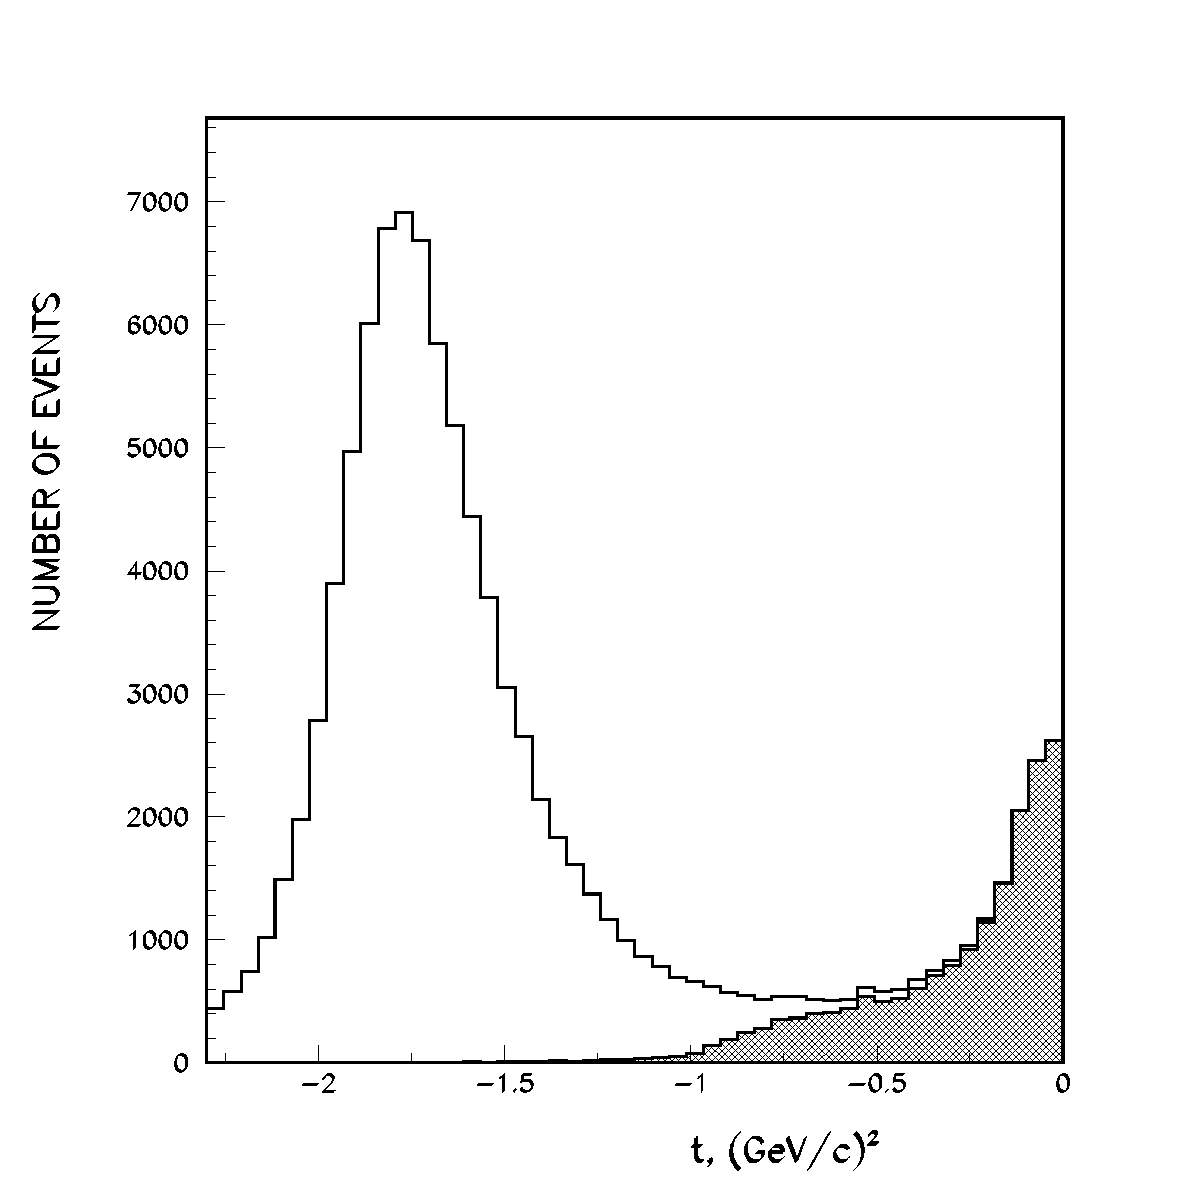
\includegraphics[width=6cm]{dist.pdf}
    %\mbox{\epsfig{figure=dist.eps,width=6.0cm}}
  \end{center}
  \vspace{0.4mm}
  \noindent
  Fig.1. The hatched area is here the charge exchange channel.\\
\end{figure}

We remind the used definition: the slowest nucleon in the deuteron rest frame is
considered as a spectator.

The operation of bubble chambers have yielded a rather valuable material of
survey character, useful for settings the purpose tasks, which, by value of
restricted statistics, it is impossible to solve with usage of a chamber
technique.

We offer to consider one of the tasks.

The speech goes about charge exchange reaction on a deuteron and its usage for
definition spin-dependent part of amplitude np$\to$pn
scattering.

At comparison differential cross sections of direct and charge exchange channels
the much the essentially different behaviour  close t=0 was remarked (Fig. 2a
and 2b).

% ******* Figure 2 *********
\begin{figure}[hbt]
  \begin{center}
    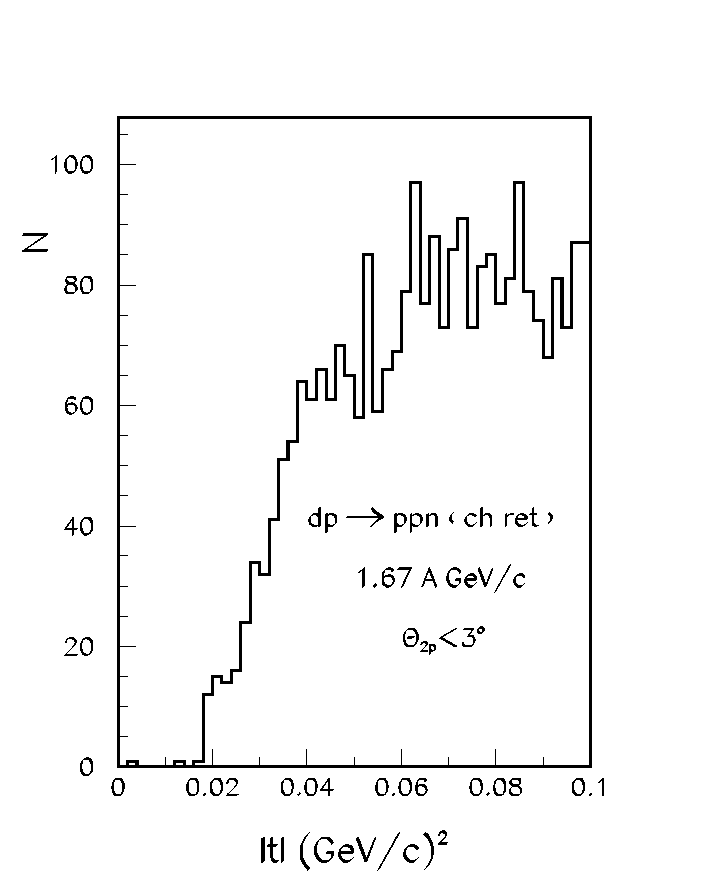
\includegraphics[width=6.5cm]{ppncrt.pdf}
    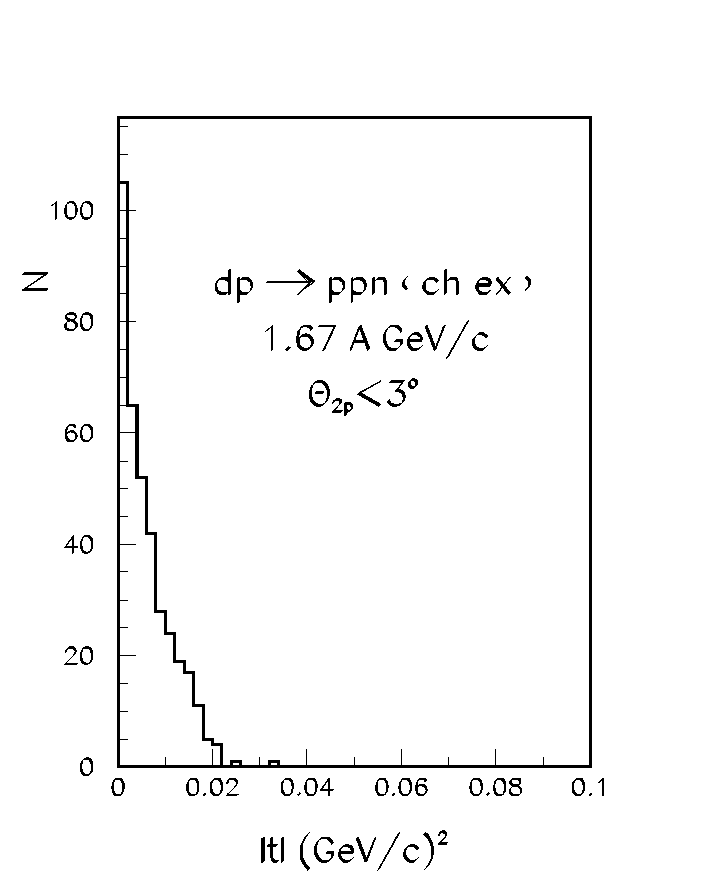
\includegraphics[width=6.5cm]{ppnce.pdf}
    %\mbox{\epsfig{figure=ppncrt.eps,width=6.cm}}
    %\mbox{\epsfig{figure=ppnce.eps,width=6.cm}}
  \end{center}
  \vspace{0,4mm}
  \noindent
  \hspace{3cm} Fig. 2a. \hspace{6cm} Fig. 2b. \\
\end{figure}


Many theorists for a long time tried to link this behaviour with the spin flip
effects.

The possibility to use the charge exchange reaction on the unpolarized deuteron
for determination of the spin dependent part of $np\to pn$ charge exchange has been
proposed by A.B. Migdal ~\cite{a2}  and I.Y. Pomeranchuk ~\cite{a3}. The
effect can be qualitatively understood in the following way. The nucleons bound
in the deuteron may be in $^{3}S_1$ and $^{3}D_1$ (T=0) spatial and spin
symmetric states but their charge states should be antisymmetric. In the charge
exchange process a charge symmetric state of two protons is produced and to
fulfill the Pauli principle at a conserved spatial symmetry, the spin flip (
$^{1}S_0$ or $^{1}D_2$ states of the two final protons) of the scattered nucleon
ensures the asymmetric total wave function.

Some words about theory:

The differential cross section of the elementary pn$\to$np charge-exchange
process may be present as sum of  the spin-independent (index1) and spin-
dependent (index2) parts:

$(d \sigma /dt)_{np\rightarrow pn}=(d \sigma /dt)_{1} +(d \sigma /dt)_{2}$.

and the amplitude of the elementary $pn \to np$ charge-exchange reaction can be
written as

$f_{ce}=a_{ce}+b_{ce} (\sigma n)( \sigma _{i}n) +c_{ce}[(\sigma n)+( \sigma _{i}
  n)]+d_{ce} [(\sigma m)( \sigma _{i}m)]+e_{ce} [(\sigma l)( \sigma _{i}l)]$,

where operators $\sigma $ and $\sigma _i$ are Pauli matrices of incident
particle (proton) and i-th nucleon (neutron) in deuteron, the coefficients
$a_{ce}$, $b_{ce}$,$c_{ce}$,$d_{ce}$,$e_{ce}$
are complex functions of interacting particles energy and scattering angle. Then
for the spin-independent and spin-dependent parts we obtain:

$(d \sigma /dt)_{1} = (\pi /p^{2}){\vert }a_{ce}{\vert }^{2}$
and
$(d \sigma /dt)_{2} =(\pi/p^{2})[ \vert b_{ce} \vert ^{2}+ \vert c_{ce} \vert
  ^{2}+ \vert d_{ce} \vert ^{2}+ \vert e_{ce} \vert ^{2}]$,
where p is the momentum in the center of mass for np-system.

The relation between the effective cross section of the deuteron peripheral
charge-exchange break-up $dp \to (pp)n$ and of the elementary $pn \to np$
charge-exchange process was discussed in the series of works~\cite{a4, a5, a6}.
Following to the mathematical formalism developed in~\cite{a4, a5}  the
differential cross section for the deuteron charge-exchange break-up reaction in
the frame of the impulse approximation can be written as:

\begin{equation}
  (d \sigma /dt)_{dp\rightarrow(pp)n} = [1-S(t)] (d \sigma /dt)_{1}+ [1-1/3S(t)]
  (d \sigma /dt)_{2}.
\end{equation}

Here
$S(t)= \int [\Psi(r)]^{2}e^{-iqr}d^{3}r$
denotes the deuteron form-factor and $t=q^2$ is the 4-dimensional transfer
momentum squared. From this formula follows that at the zero transfer momentum
from proton-target to neutron, i.e. at the zero scattering angle, because of
S(0)=1, the differential cross section (1) equals to:

\begin{equation}
  (d \sigma /dt)_{dp\rightarrow(pp)n} = 2/3 (d \sigma /dt)_{2}.
\end{equation}

Thus, the charge-exchange break-up reaction of the unpolarized deuteron on the
unpolarized proton-target in the forward direction is completely determined by
the spin-flip part of the elementary $np \to pn$ charge-exchange process at the
zero scattering angles. So, deuteron behaves itself as a spin filter. It should
be noted that the result (2) also remains valid when the deuteron D-state is
taken into account.

At the forward scattering $\vert c_{ce}\vert ^2 = sin^2 \theta =0$ and
$\vert b_{ce}-d_{ce}\vert ^2 = sin^2 \theta = 0$.

Consequently for the forward scattering we obtain:

\begin{equation}
  (d \sigma /dt)_{dp\rightarrow(pp)n} = 2/3 (\pi/p^{2})[ 2\vert b_{ce}%
    \vert ^{2}+ \vert e_{ce} \vert ^{2}].
\end{equation}

So the study of the process $dp\to (pp)n$ at small transfer momentum allows to
estimate the spin-flip part of the amplitude of the elementary $np\to pn$
reaction, i.e. sum of amplitudes $2\vert b_{ce}\vert ^2+\vert e_{ce}\vert ^2$.

The last formula is applicable if at least two conditions are fulfilled:

\begin{enumerate}
\item the momentum transfer of the quasielastic np scattering is small,
\item the intrinsic momenta q of the nucleons in the deuteron are small.
\end{enumerate}

The second condition means S-wave dominance in the deuteron wave function. It
can be seen, e.g. in Fig 3, where the S wave probability distribution is shown
as a function of the nucleons intrinsic momenta. In the region below p=0.07
GeV/c this probability practically does not depend on the nucleon intrinsic
momenta.

% ******* Figure 3 *********
\begin{figure}[hbt]
  \begin{center}
    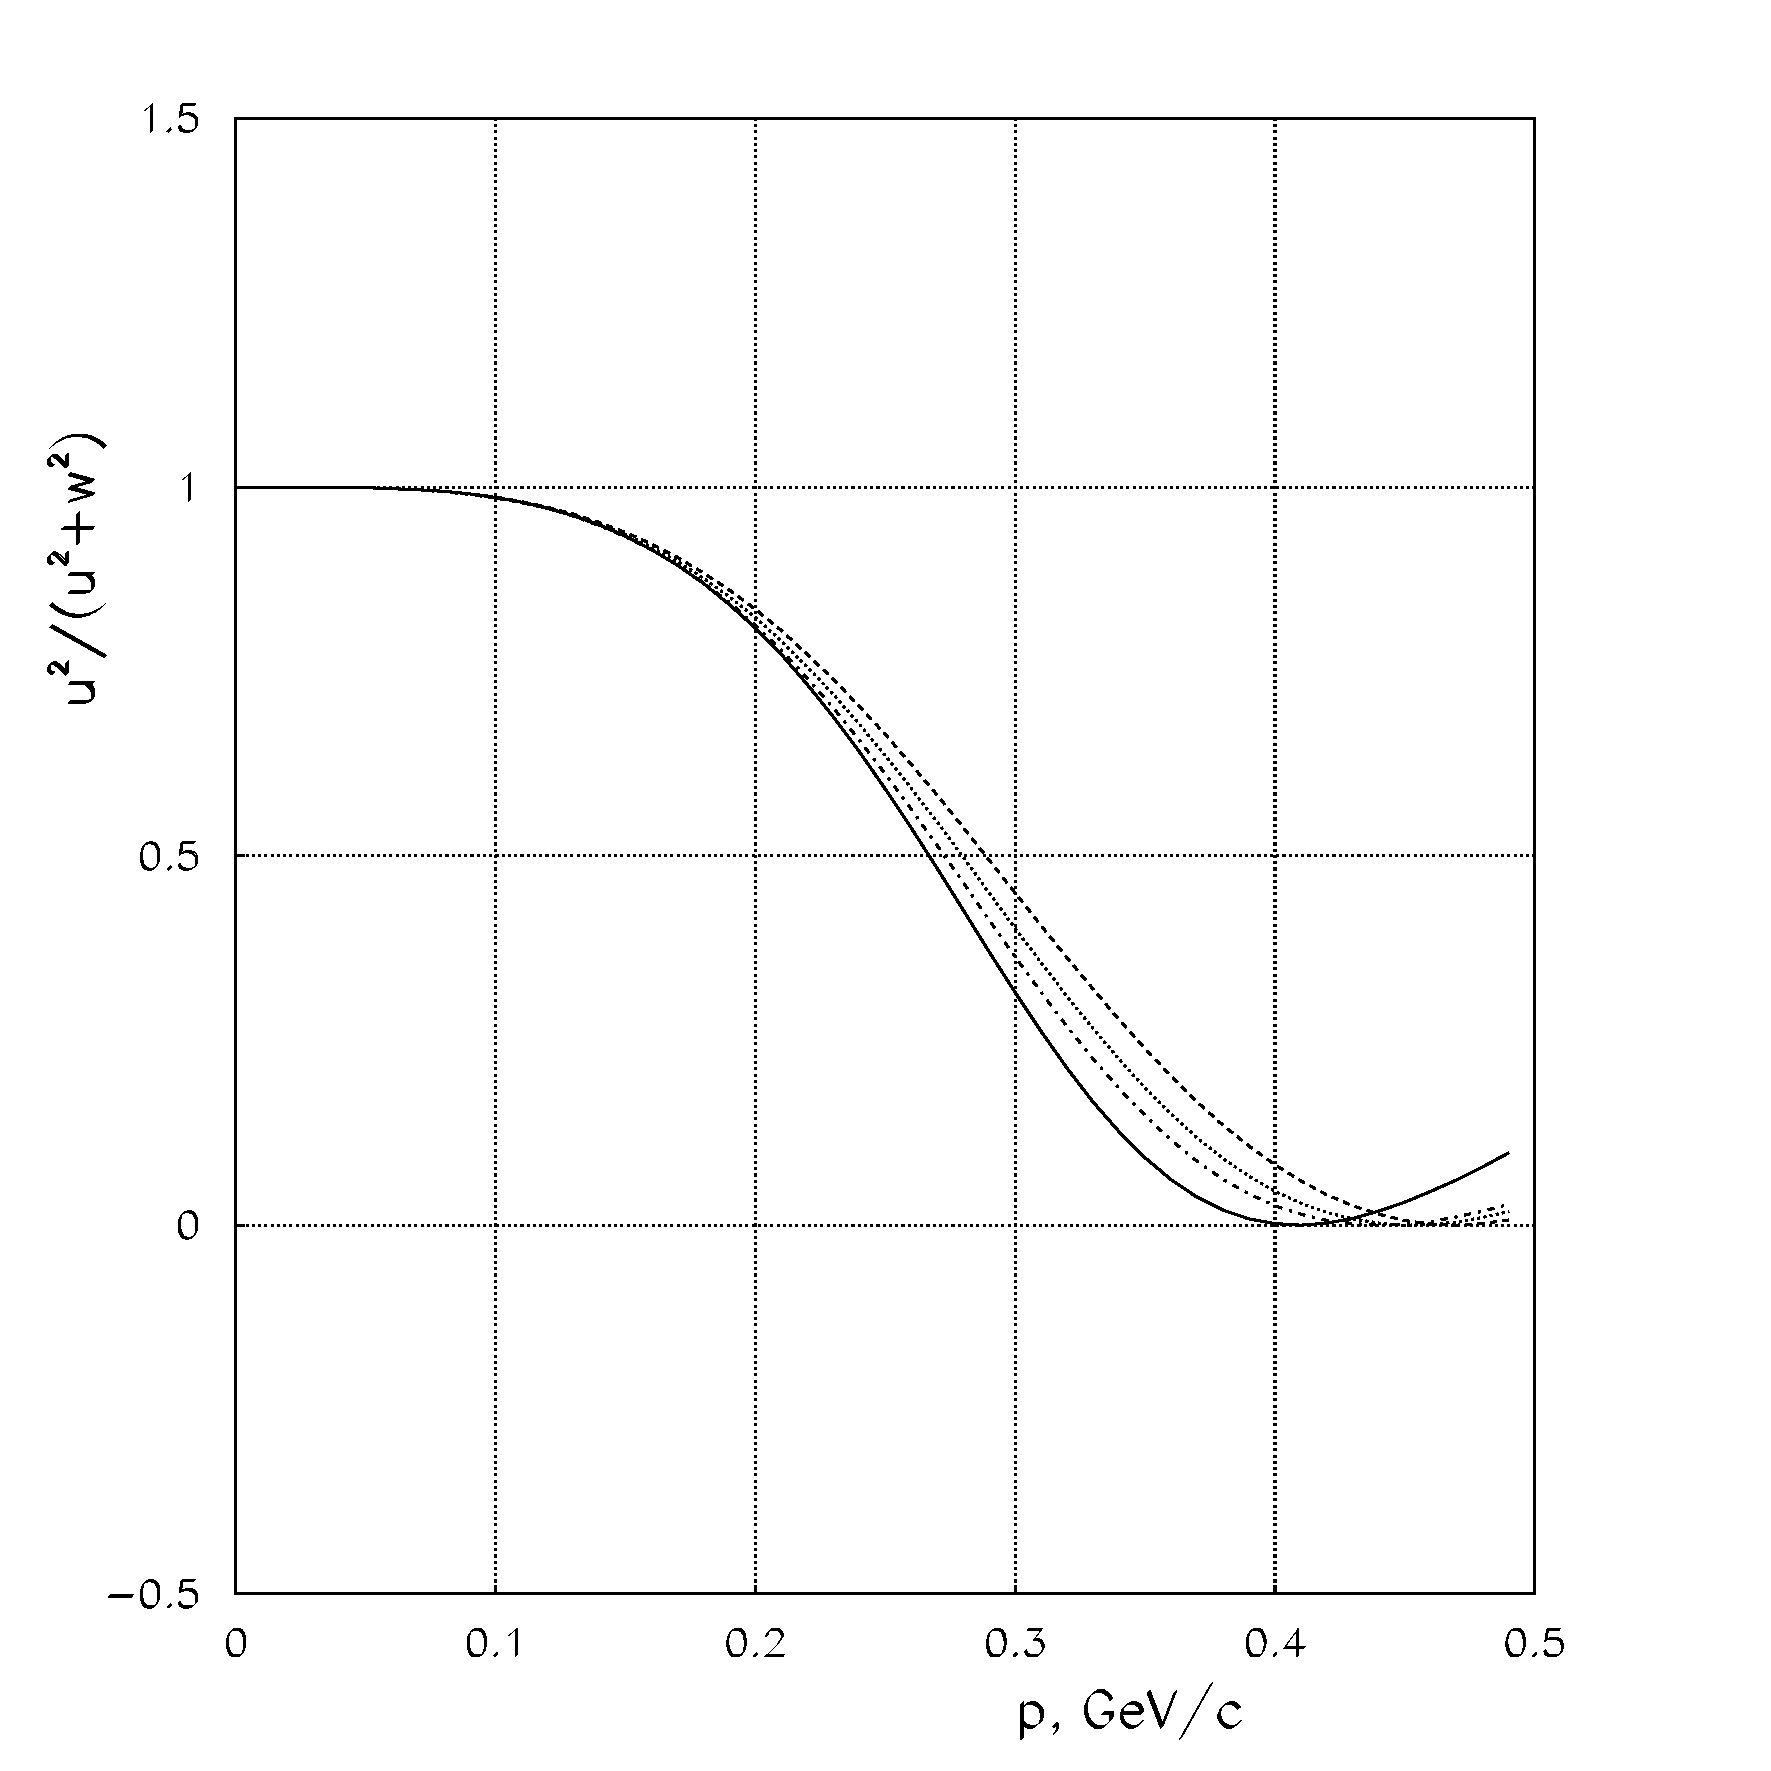
\includegraphics[width=6.5cm]{wavedtr.pdf}
    %\mbox{\epsfig{figure=wavedtr.eps,width=6.cm}}
  \end{center}
  \vspace{0,4mm}
  \noindent
  Fig. 3. The S wave probability as a function of the nucleon Fermi momentum. \\
\end{figure}

Both the above mentioned conditions can be fulfilled simultaneously, if one
selects events in the laboratory frame ( fast deuteron impinges on the proton
target ) containing two fast protons  at small production angle, with momentum
close to the half of the deuteron's one. We would like to emphasize, that this
task can be realized successfully in the beams of accelerated deuterons. In the
case of a deuteron target the two protons are too slow to be detected and the
reaction cannot be identified.

To answer the question of the spin flip contribution of the np$\to$pn
process as it follows from expression (2), it is necessary to turn to the
experimental data on np$\to$pn
charge exchange differential cross section at t=0. Such data have been obtained
at Brookhaven [7] for
the region of 1-8 GeV and could be reasonably approximated by the function
$1/p^2$, where p is the momentum of the incoming neutron (Fig.4). The data imply
$(d\sigma /dt)(0) = (36.9 \pm 3.0)$ (GeV/c)$^2$ at 1.67 GeV/c. Now the task is
to compare the differential cross section of the exchange on the deuteron,
obtained in our experiment at t=0 with those for the np$\to$pn
at the corresponding beam energy.

% ******* Figure 4 *********
\begin{figure}[hbt]
  \begin{center}
    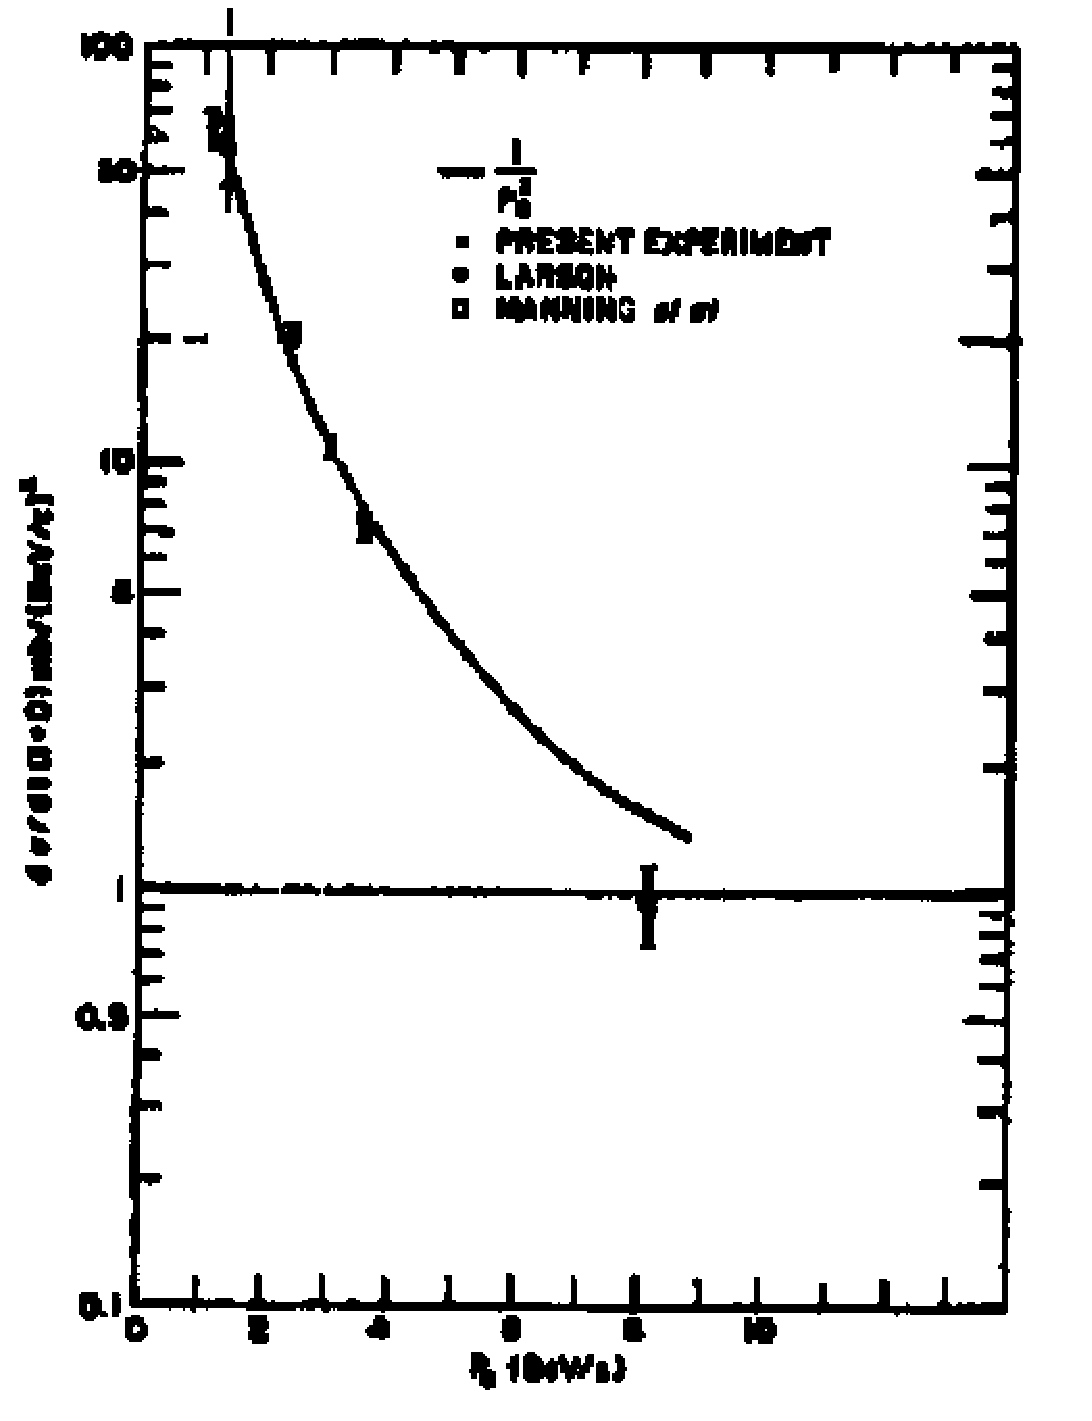
\includegraphics[width=6cm]{fig4.pdf}
    %\mbox{\epsfig{figure=fig4.eps,width=6.cm}}
  \end{center}
  \vspace{0,4mm}
  \noindent
  Fig.4. Charge exchange channel np$\to$pn
  differential cross section at t=0.\\
\end{figure}

The relation between these two reactions in the case of polarized deuteron beam
is considered in~\cite {a8}. According to this work using of the polarized
deuterons allows one, in principle, to separate two spin-dependent terms in the
amplitude of the charge-exchange reaction np$\to$pn, one of each (proportional
to $b_{ce}$) does conserve and the other one (proportional to $e_{ce}$)
conserves the projection of the nucleon spin onto the direction of momentum at
the transition of neutron into proton.

In future charge exchange reaction of polarized deuteron on the polarized proton
target under 0 degrees will allow to define a relativistic phase of two
indicated amplitudes, that is so lead "complete experience".

We have begun similar experiment in Dubna (LHE JINR) with the help of setup
STRELA on the new superconducting accelerator NUCLOTRON~\cite {a9}.

STRELA is very simple installation for measurements of an exit of pairs of
protons from dp-interactions with momentum 0.5 of beam momentum under zero
degrees.

We have the next problem:

Difficulty of selection of protons pairs from background of major number of
single proton, which at the aperture of 0.2 degrees makes approximately 4000 per
one pair of protons. The experimental scheme, presented in fig. 5 will be used.

% ******* Figure 5 *********
\begin{figure}[hbt]
  \begin{center}
    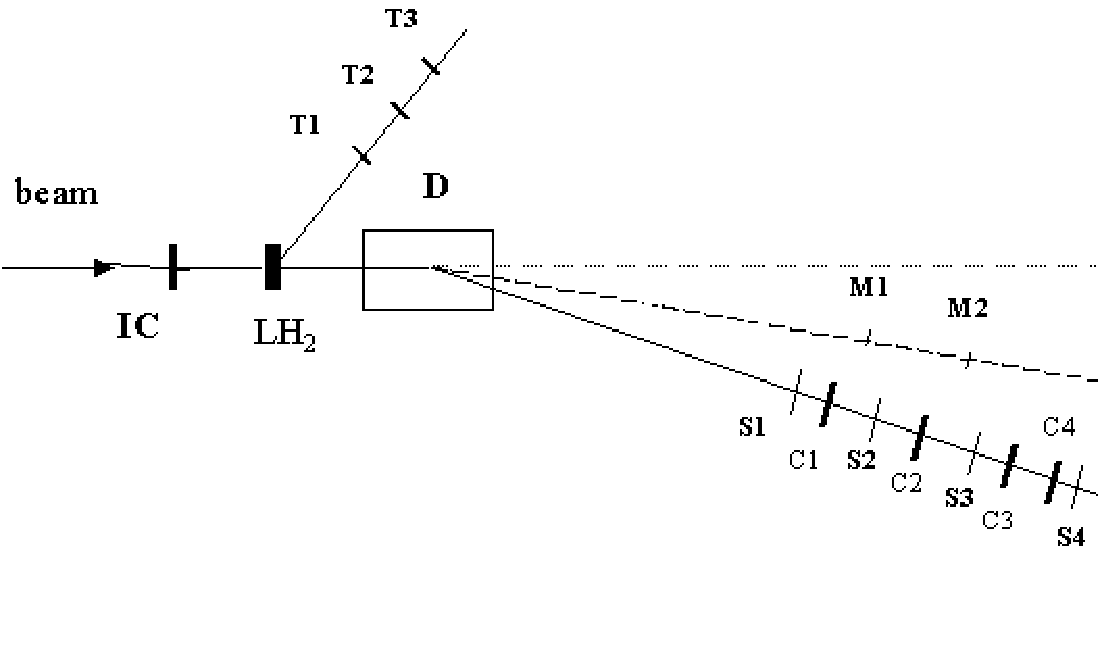
\includegraphics[width=9cm]{image2.pdf}
    %\mbox{\epsfig{figure= image2.eps,width=8.cm}}
  \end{center}
  \vspace{0,4mm}
  \noindent
  Fig.5. Experimental scheme of Strela setup \\
\end{figure}

The slow extraction deuteron beam is incident on a 10-cm liquid hydrogen
target
LH$_2$ and the analyzing magnet D separates the primary deuterons and
secondary
particles. The ionization chamber IC measures a flux of the deuteron
beam. The
scintillation monitors T1-T3 and M1-M2 control the intensity and position
of the
beam. The scintillation counters S1-S4 with diameters of 48 mm determine the
angular $(\sim 0.2^0)$ and momentum $(\sim 10\%)$
acceptance and trigger of the events.
The Cherenkov counters C1-C3 with sapphire radiators of the size
50x50x16
$~mm^{3}$
select the two-proton events. The expected resolution about $\sim9\%$
allows to separate reliably the two and one-proton events.

In March of this year the first run of setup  Strela  was made at normal
parameters of a
deuteron beam and with  liquid hydrogen target.   On the diagram (Fig.6.)   the
correlation of amplitudes  from two Cerenkov counters is shown at momentum of
deuteron beam 4.0 GeV/c.  Except for a ground  mass  of one-proton events (area
of small amplitudes) the accumulation of points is visible at major amplitudes.
On a projection at exception of one-proton events (Fig.7) two maximums are well
visible.  The maximum at  the greater amplitude corresponds to an output of
narrow proton pairs.

% ******* Figure 6 *********
\begin{figure}[hbt]
  \begin{center}
    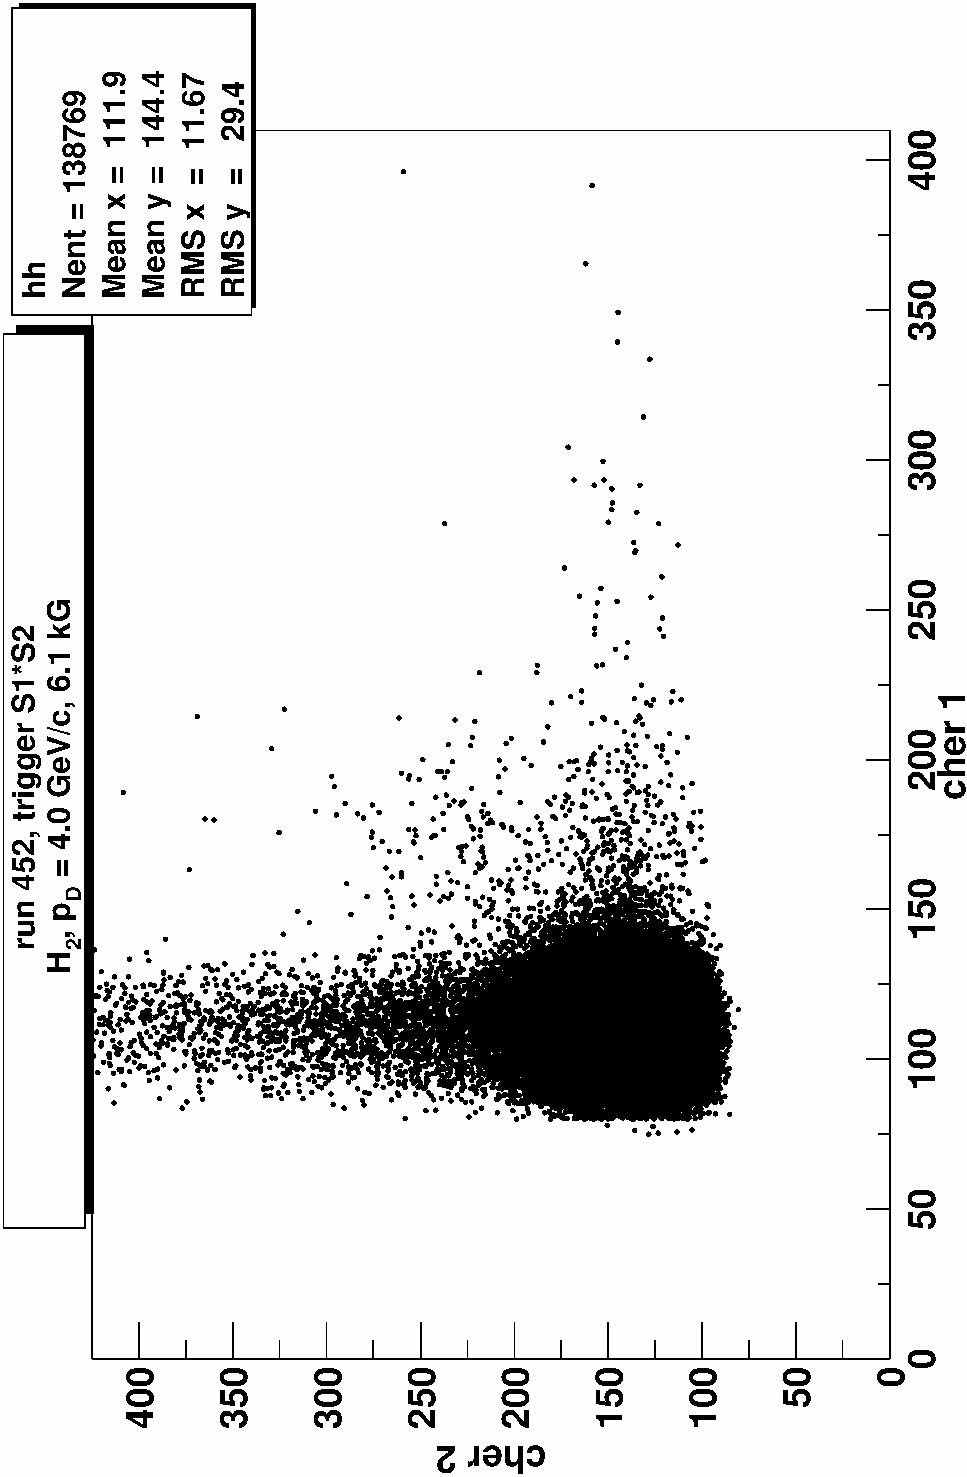
\includegraphics[width=5.3cm,angle=270]{plot.pdf}
    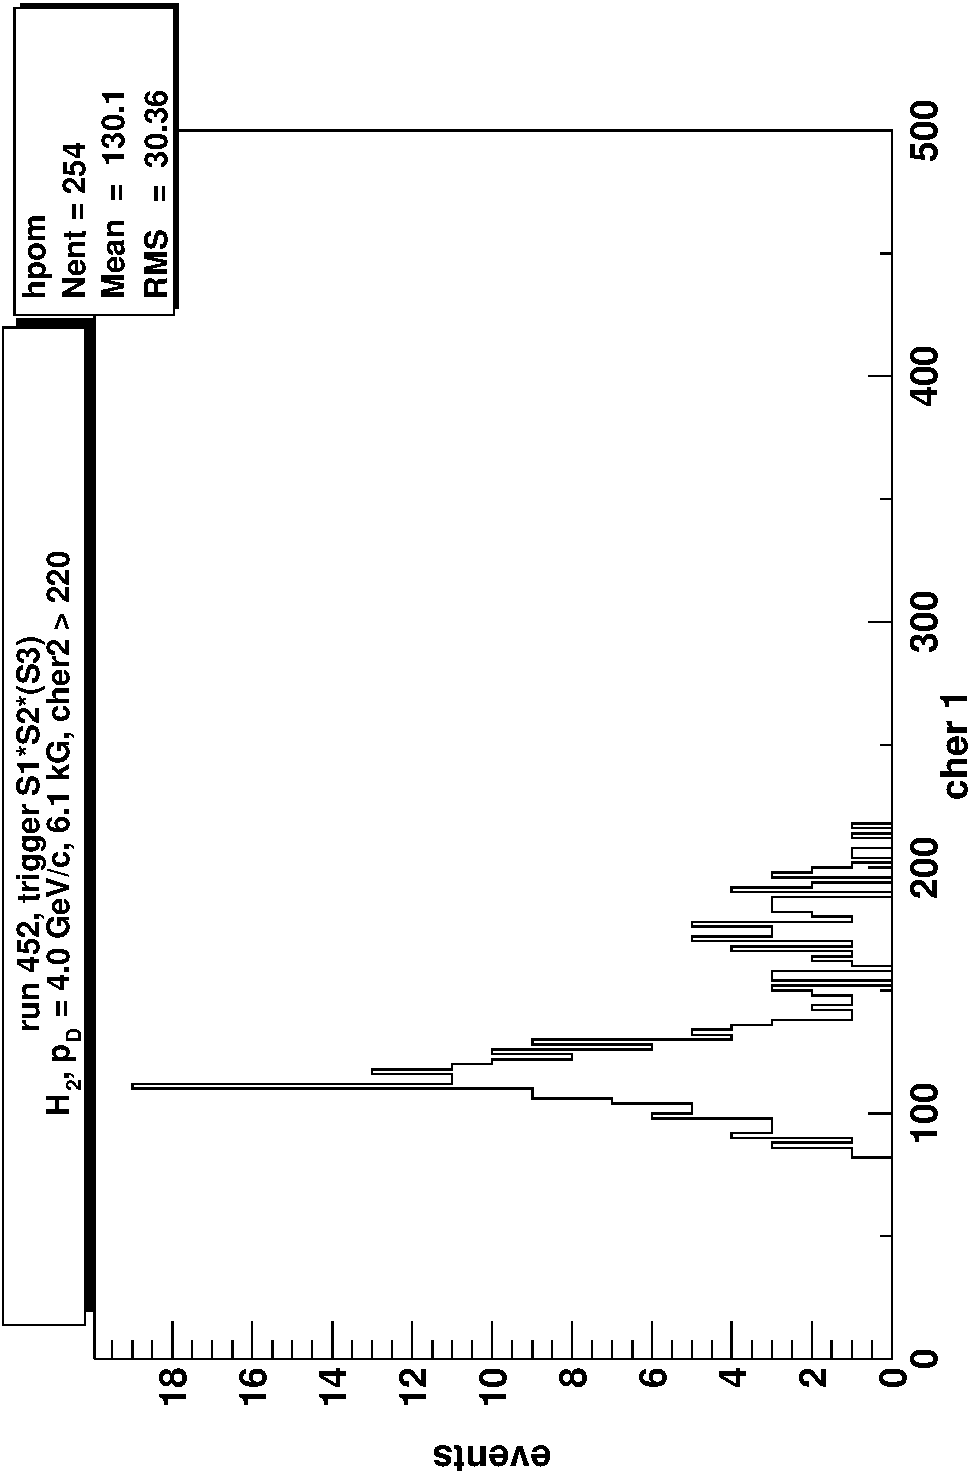
\includegraphics[width=5.3cm,angle=270]{proj.pdf}
    %\mbox{\epsfig{figure= plot.eps,width=6.cm,angle=270}}
    %\mbox{\epsfig{figure= proj.eps,width=6.cm,angle=270}}
  \end{center}
  \vspace{0,4mm}
  \noindent
  \hspace{3cm} Fig.6.\hspace{6cm} Fig.7 \\
\end{figure}


The tentative estimation of the ratio of number of pairs of protons to an one-
proton background if take in account effect of an empty target, efficiency of
selection, and also dependence  of the cross section  of the charge-exchange
np$\to$pn reaction at 0 degrees from energy yields the value
$1/3400 (0.00029\pm0.00006)$.

Calculation of Monte-Carlo (GEANT) with usage on an input of real events from
the hydrogen bubble chamber~\cite{a10} , in view of geometry of setup STRELA
have yielded $1/3200 (0.00031\pm 0.00006)$.

Closeness of these ratios (at an error about 20\% from behind small statistics)
specifies the major contribution spin dependent part of amplitude of np$\to$pn
charge exchange reaction.

In next run of the Nuclotron the parameters of Strela setup will be improved.
In particular, its aperture will be enlarged, that  will be risen by efficiency
of an output of proton pairs in 3-4 times.

\begin{thebibliography}{99}

\bibitem{a1} V. V. Glagolev, Nucl. Phys. B (Proc. Suppl.) 36 (1994) 509-512
\bibitem{a2} A. B. Migdal, Sov. JETF 28 (1955) 3
\bibitem{a3} ] I. Pomeranchuk, Sov. JETF 21 (1951) 1113
\bibitem{a4} L. Lapidus, Sov. JETF 32 (1957) 1437
\bibitem{a5} N. W. Dean, Phys. Rev. D5 (1972) 1661; Phys. Rev. D5 (1972) 2832
\bibitem{a6} D. V. Bugg, C. Wilkin, Nucl. Phys. A467 (1987) 575
\bibitem{a7} J. L. Friedes et al., Phys. Rev. Lett. I5 (1965), 38-41
\bibitem{a8} V. V. Glagolev et al. JINR E1-99-280, Dubna, 1999
\bibitem{a9} Yu. P. Bushuev et al., Proc. of the Int. Workshop "Relativistic
  nuclear physics: from hundreds MeV to TeV", Slovak Republic, Stara Lesna 2000,
  Dubna, JINR, 2001, pp. 234-245
\bibitem{a10} V.V. Glagolev et al., Particles and Nuclei, Letters N3[100]-
  2000,pp. 67-73

\end{thebibliography}
\end{document}
